\documentclass[border=0cm]{standalone}
\usepackage{tikz}
\usetikzlibrary{arrows, arrows.meta}

\tikzset{
    node1/.style={
        above right
    }
}
\begin{document}
    \begin{tikzpicture}
        \node at (0,27)  {\Huge (a)}; \node[node1] at (1,15)   {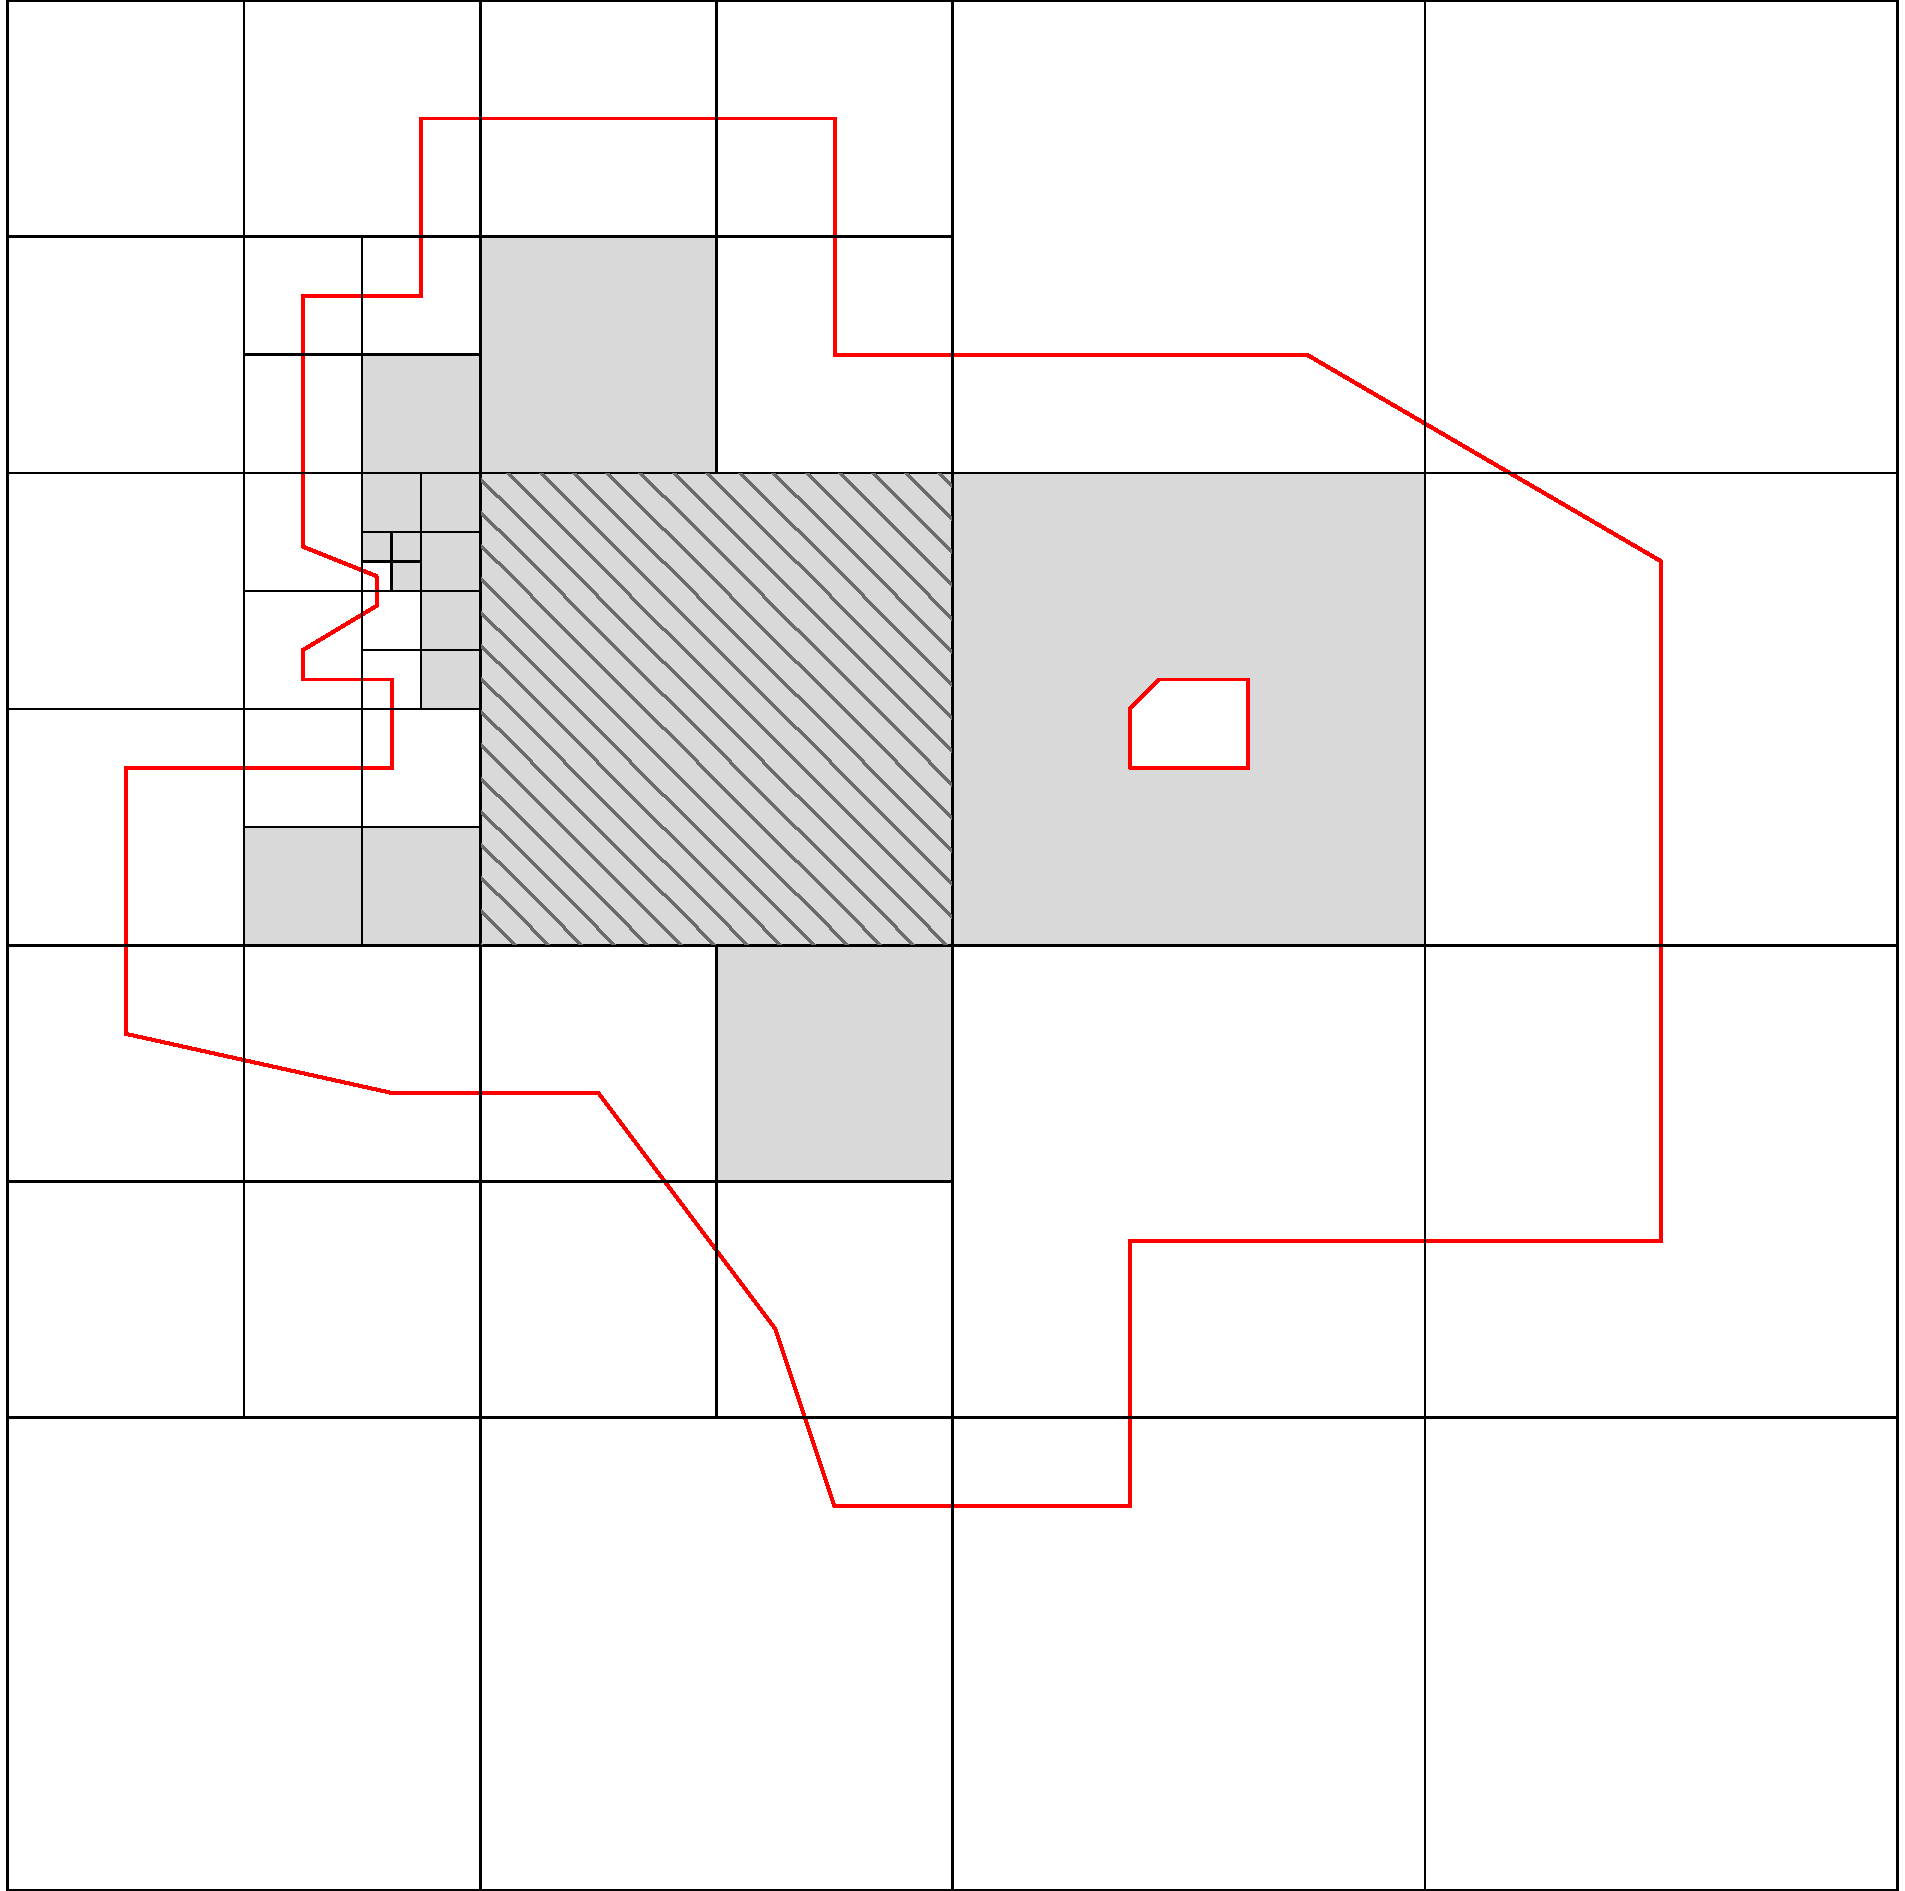
\includegraphics[scale=0.4]{emptycells}};
        \node at (15,27) {\Huge (b)}; \node[node1] at (16,15)  {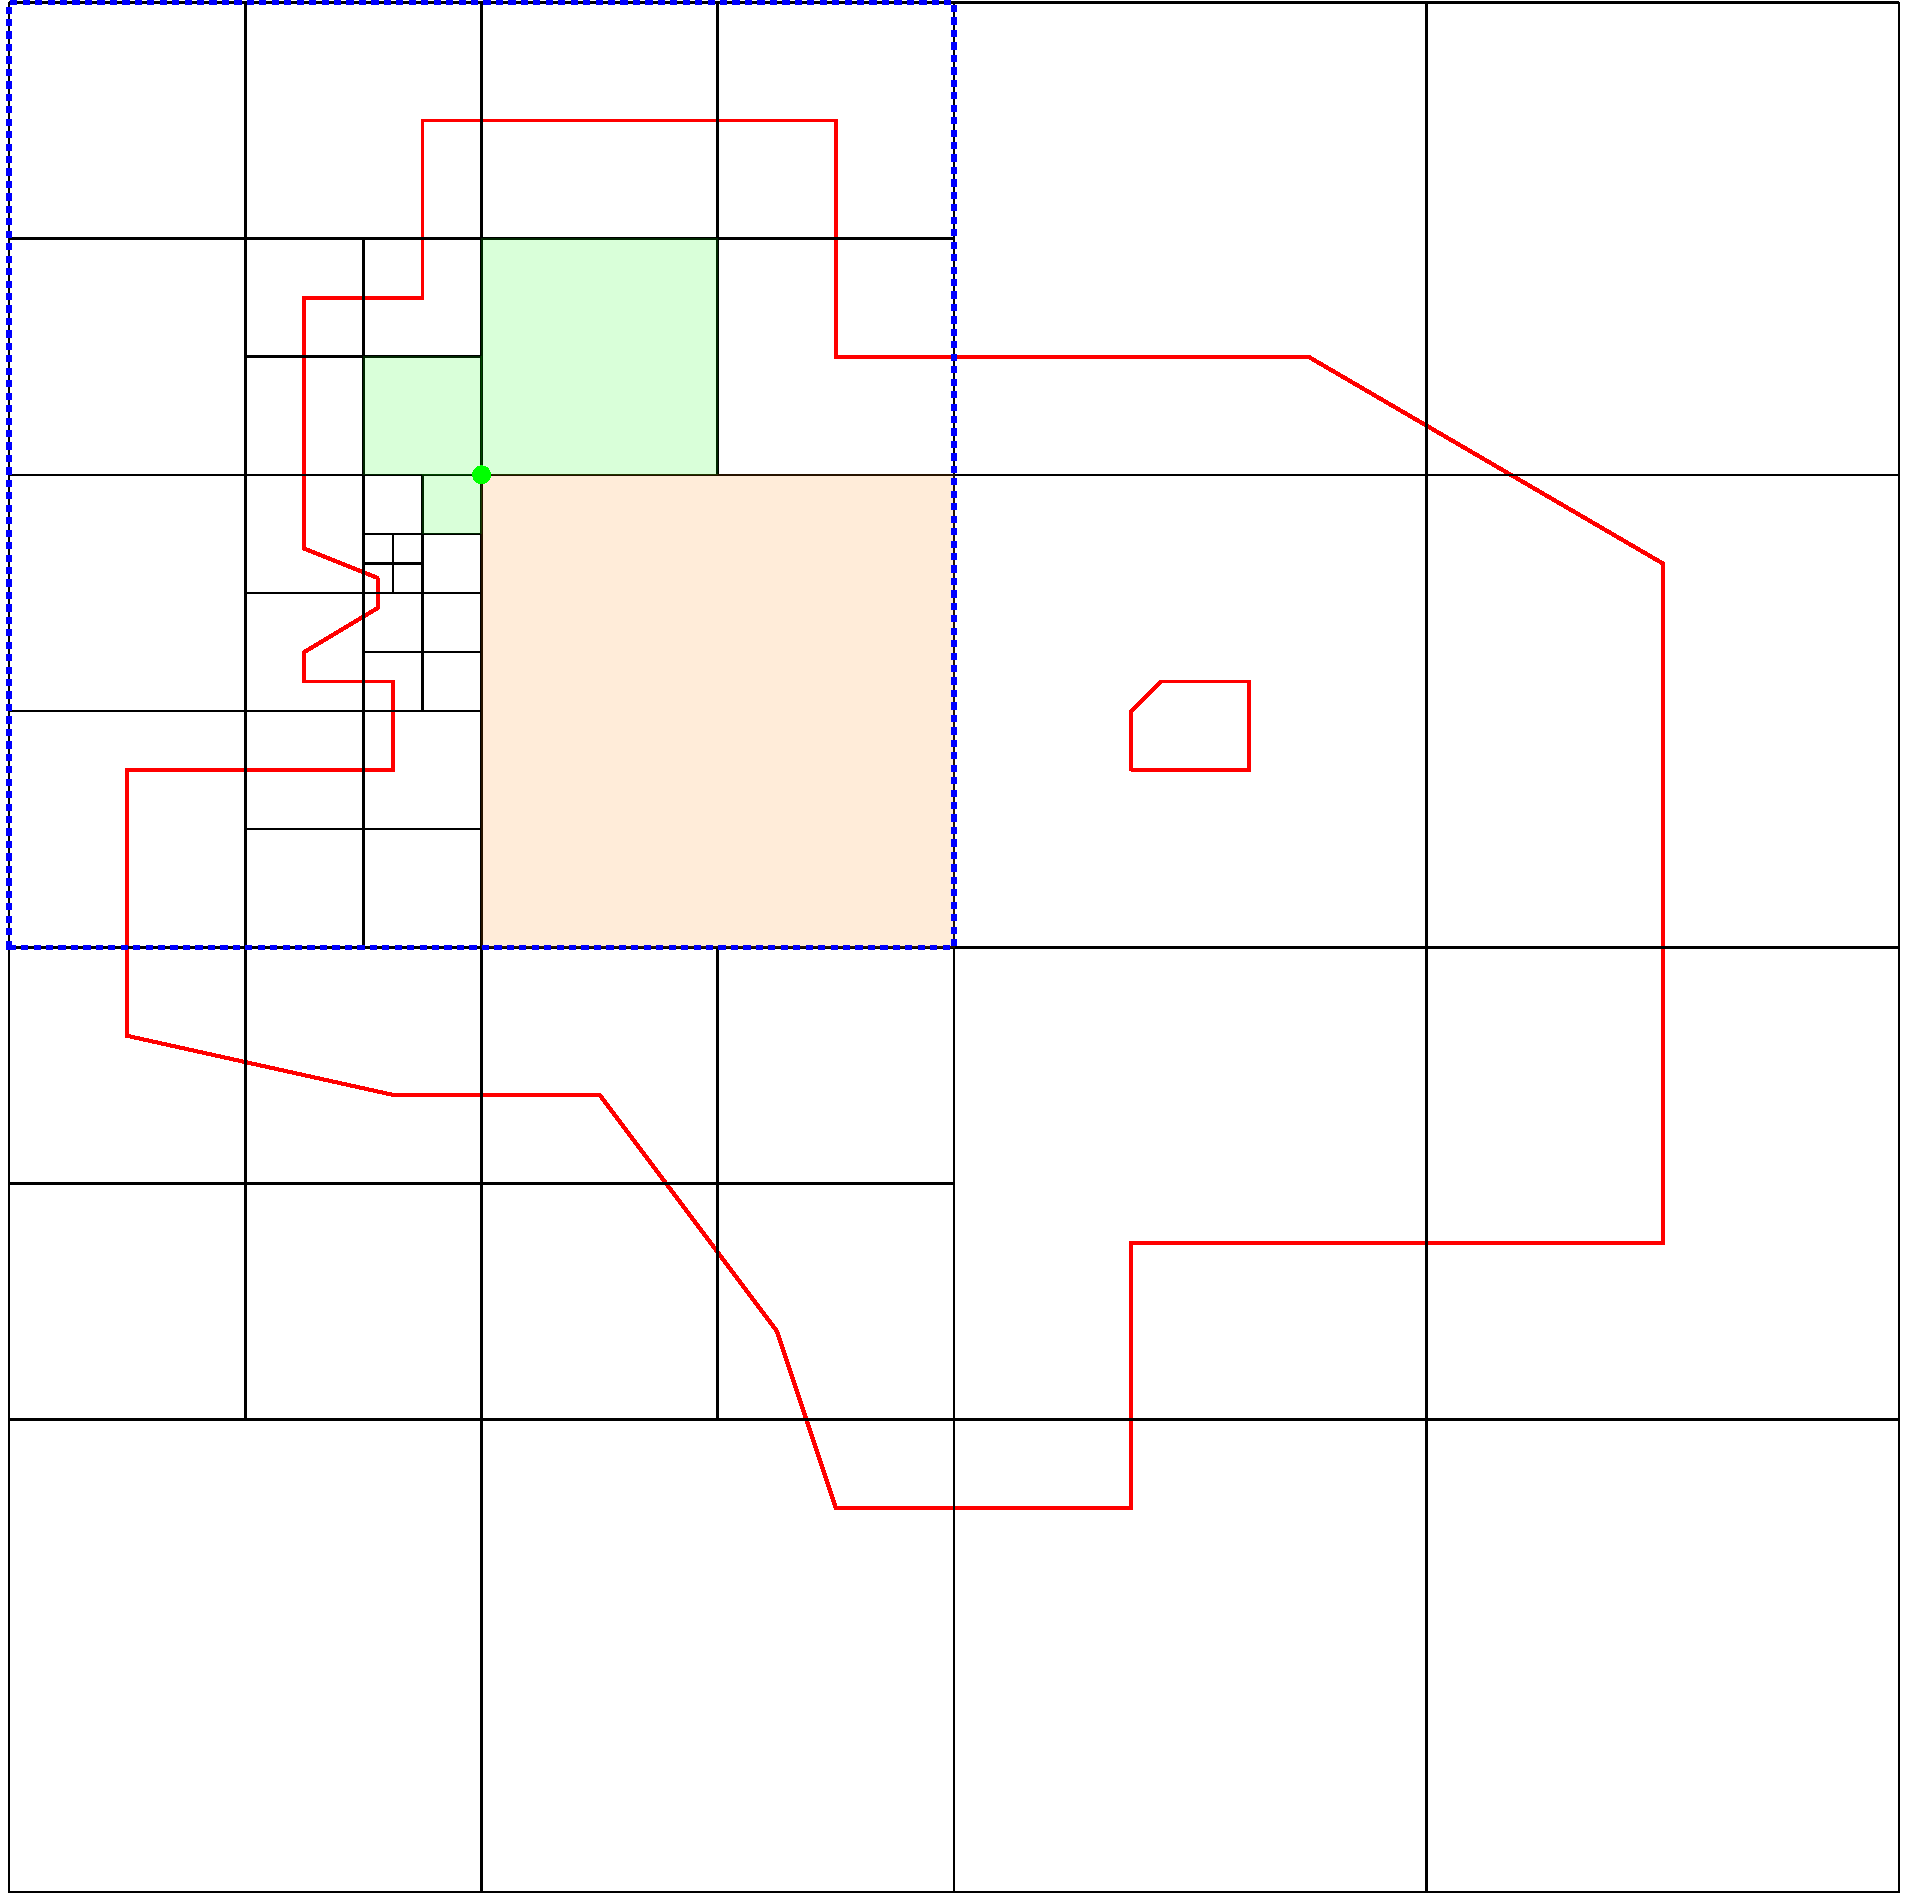
\includegraphics[scale=0.4]{example1}};
        \node at (0,13)  {\Huge (c)}; \node[node1] at (1,1)    {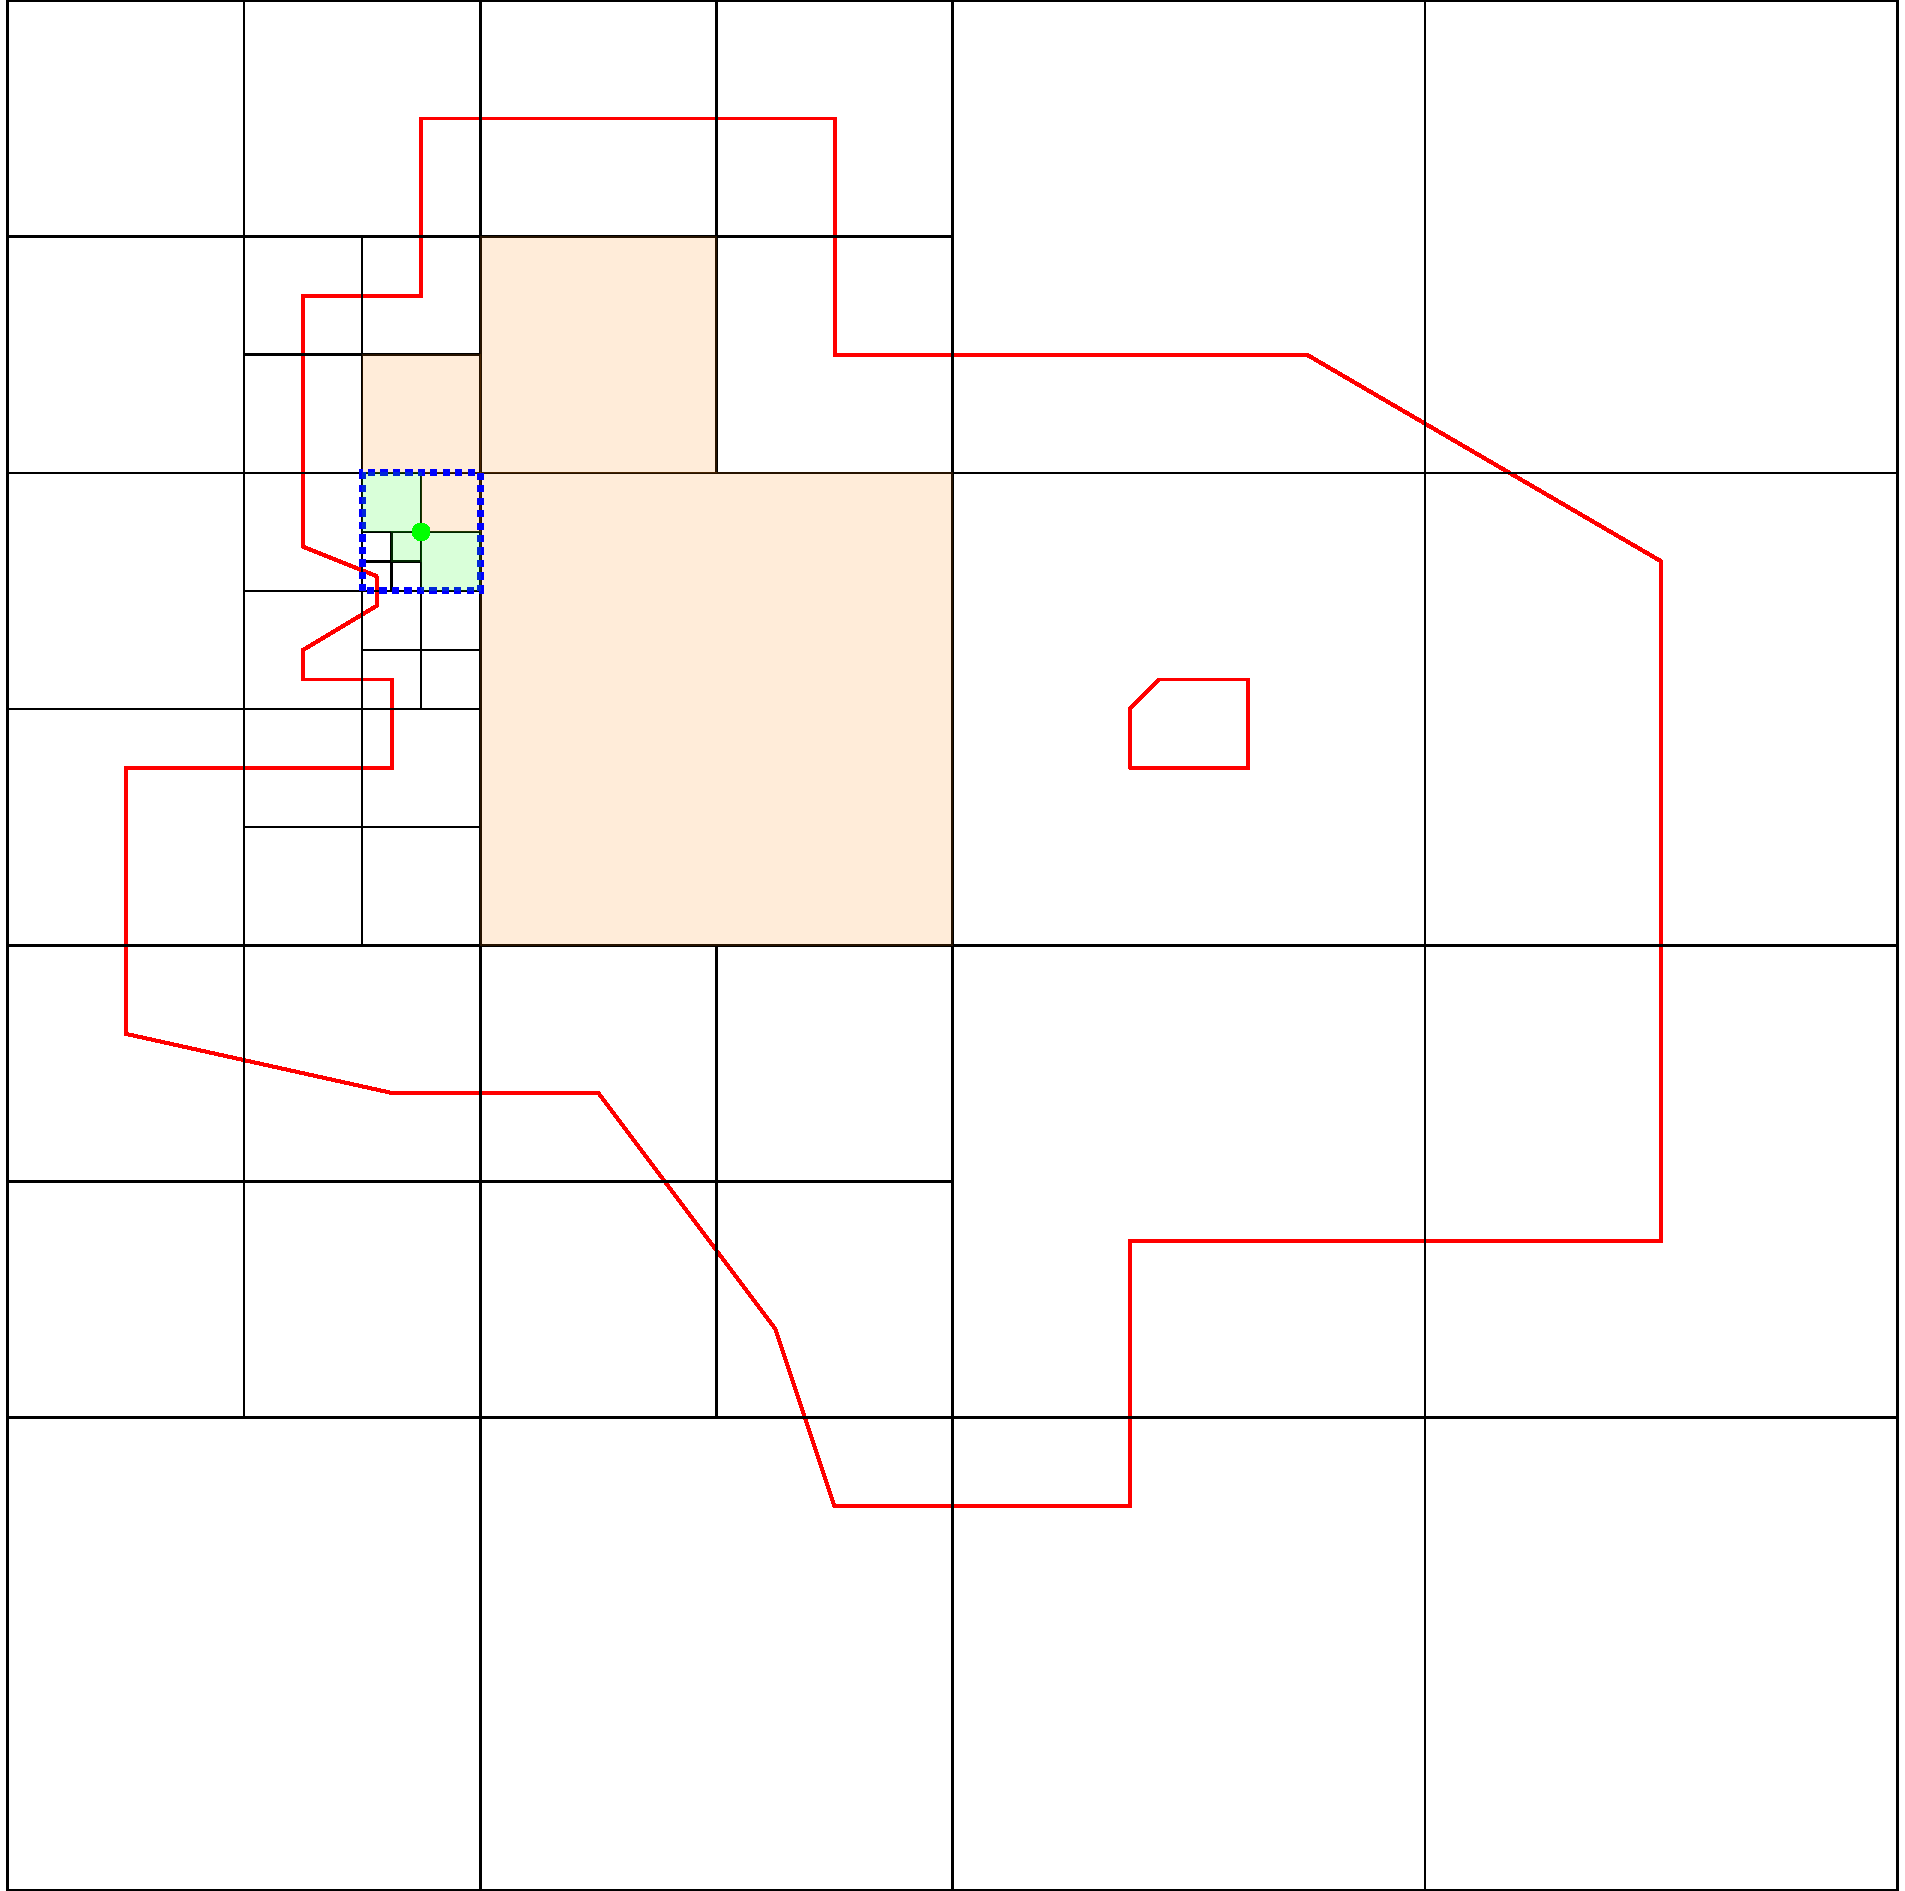
\includegraphics[scale=0.4]{example2}};
        \node at (15,13) {\Huge (d)}; \node[node1] at (16,1)   {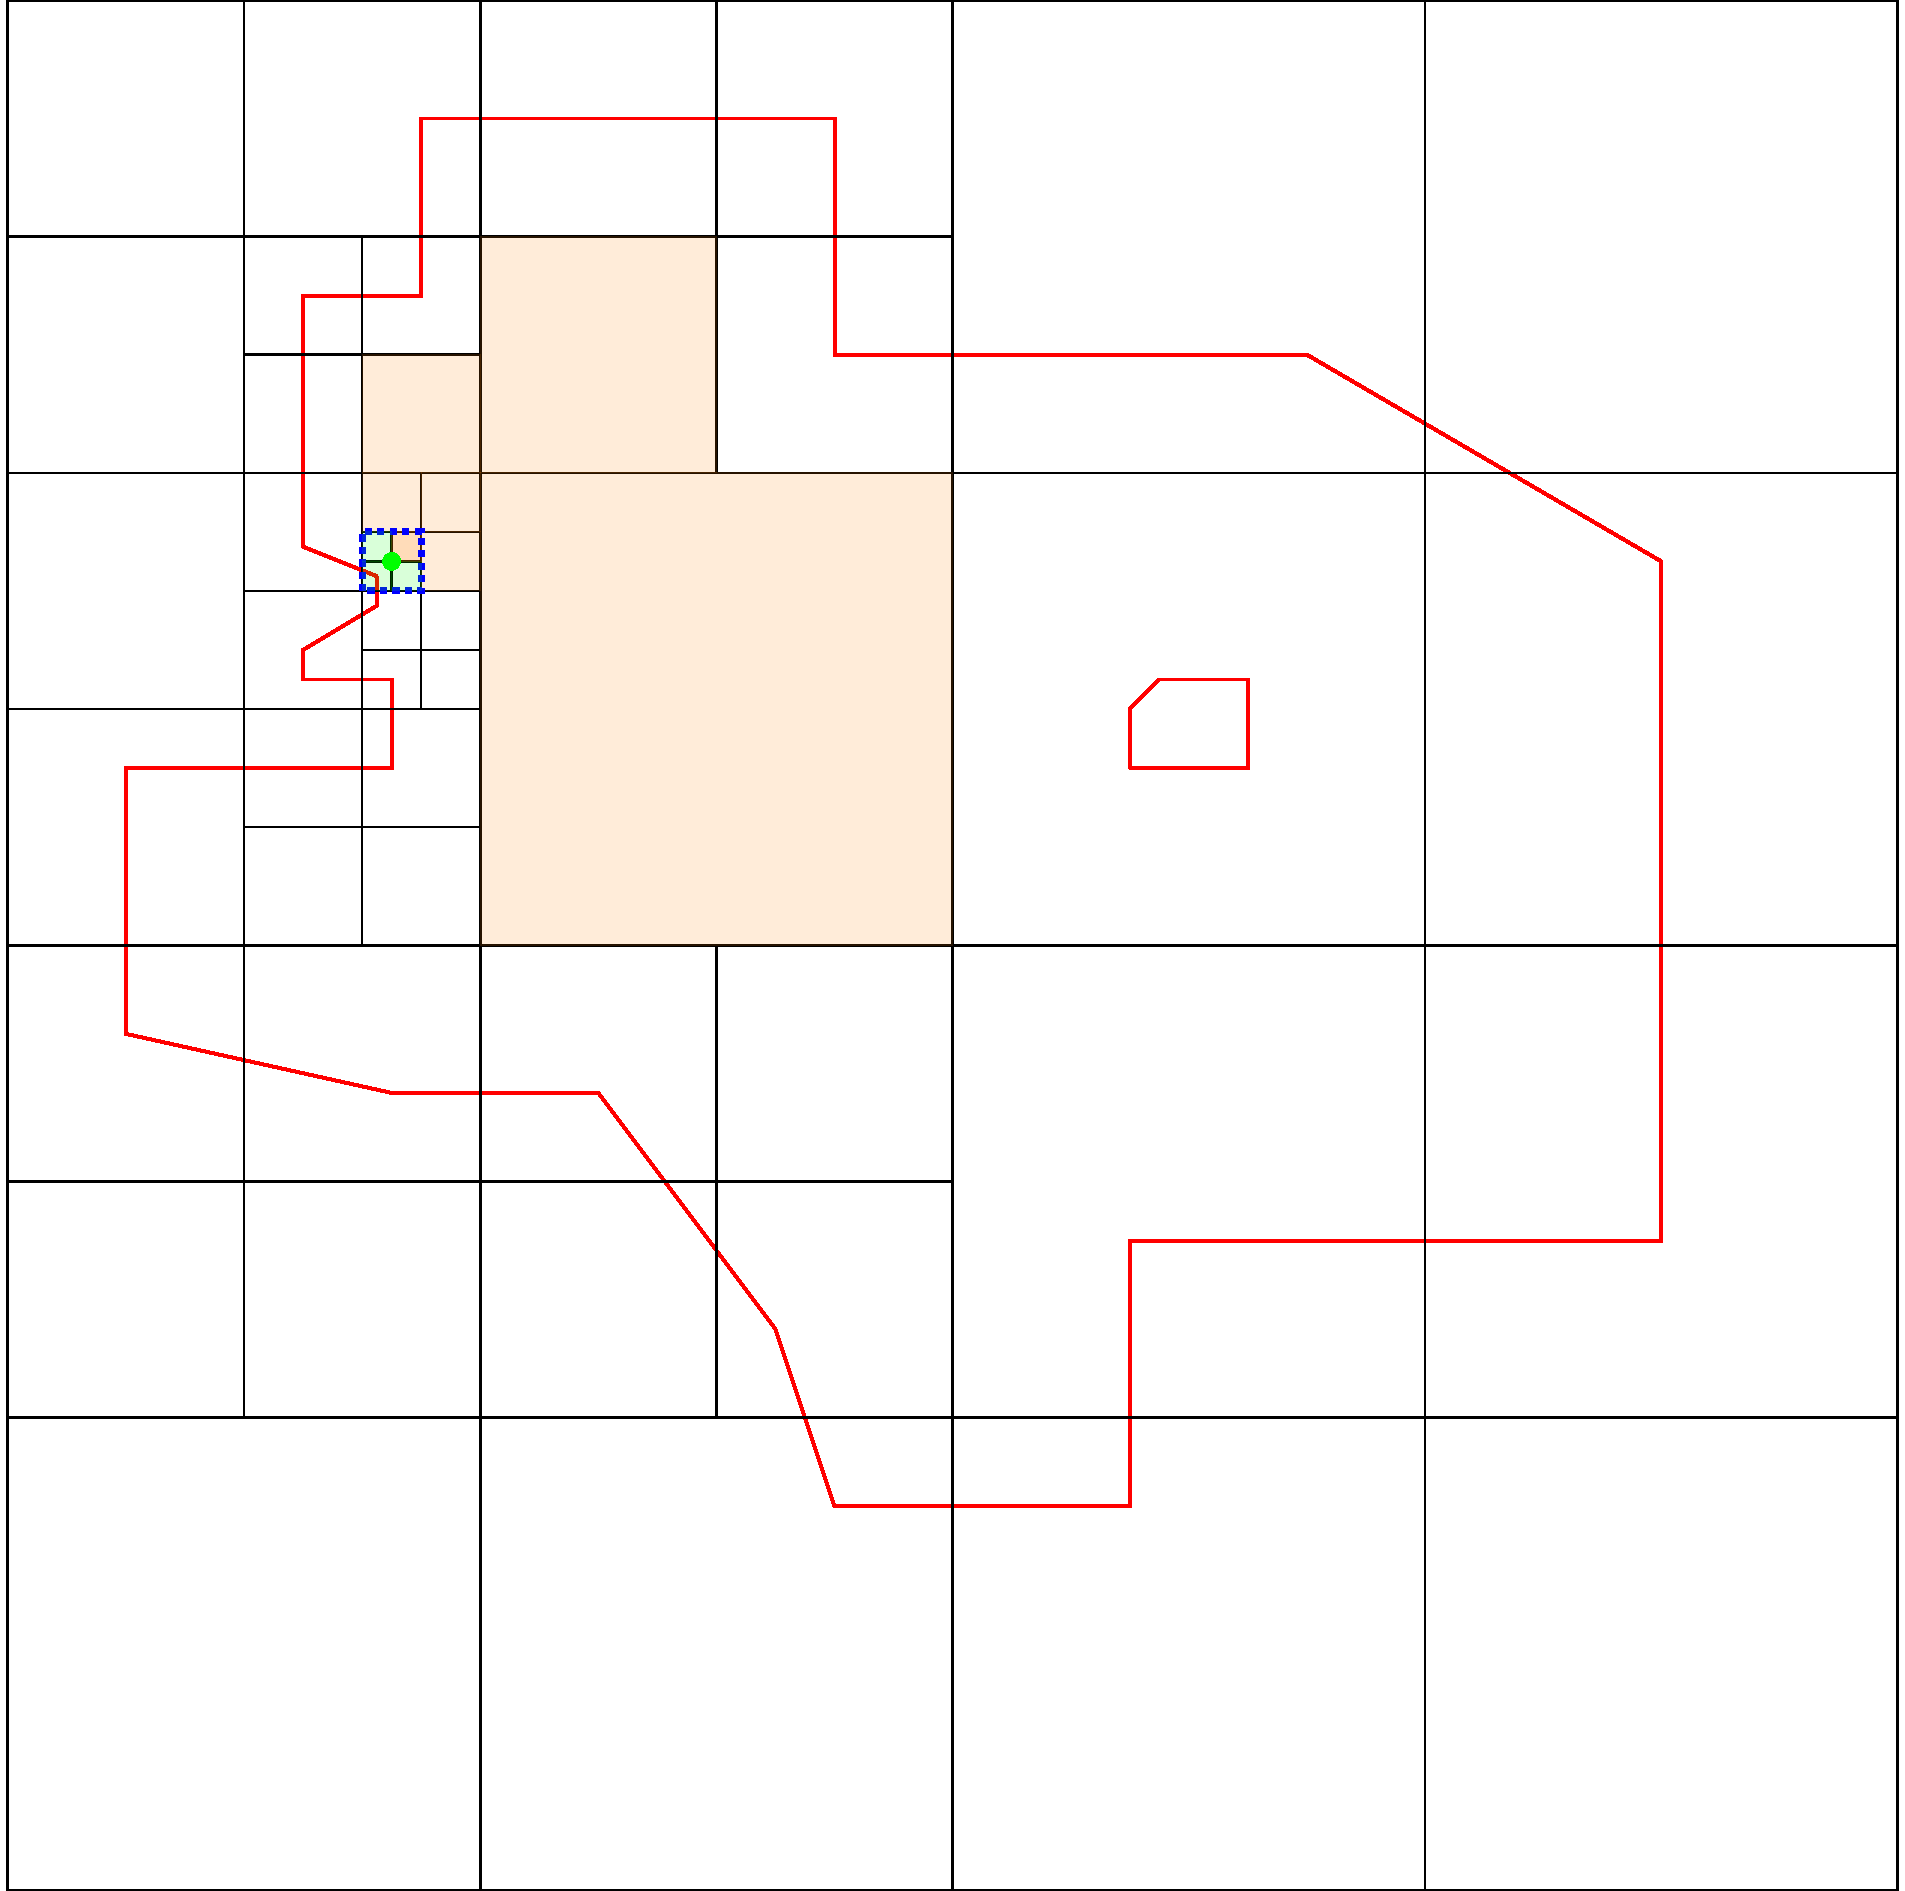
\includegraphics[scale=0.4]{example3}};
    \end{tikzpicture}
\end{document}
